\newcommand{\ClassPath}{../../yukibook.cls}
\documentclass{\ClassPath/yukibook}


\begin{document}

    \yukibook{Introducción a Laravel} % Title
    {Rubén Gómez Olivencia}  % Author
    {2023}    % Year
    {} % Name of degree
    {} % catch phrase
    {} % the phrase's author
    {img/logo.png} %cover
    {ff5449}
    {} %mini-title

    \coverpage
    \graphicspath{{../../yukibook.cls/}}
    \licensepage
    %
    \tableofcontents

    %--------------------------------------------------------------------------
    % Start your parts, chapters and sections here
    %--------------------------------------------------------------------------
    \graphicspath{{img/}}

    \part{Introducción}
    \chapter{Introducción a Laravel}

\href{https://laravel.com/}{Laravel} es un \textit{framework} para crear aplicaciones y servicios web haciendo uso del lenguaje de programación \href{https://es.wikipedia.org/wiki/PHP}{PHP}, buscando la simplicidad y evitar el “\textit{spaghetti code}”. Hace uso de la arquitectura “modelo-vista-controlador” (MVS) y es un proyecto de código abierto.

\section{Características}
Entre las características que tiene Laravel, se pueden destacar:

\begin{itemize}
    \item Sistema de enrutamiento, también RESTful.
    \item Motor de plantillas web llamado \href{https://laravel.com/docs/10.x/blade}{Blade}. Nos permite:
    \begin{itemize}
        \item Crear plantillas que pueden incluir otras plantillas.
        \item Hacer uso de PHP dentro de las plantillas.
        \item Permite cachear las plantillas hasta que se modifiquen.
    \end{itemize}
    \item Creador de queries a la base de datos llamada \href{https://laravel.com/docs/10.x/queries}{Fluent}.
    \item \href{https://laravel.com/docs/10.x/eloquent}{Eloquent} como ORM (\textit{object-relational mapper}).
    \item Uso de “\textit{migrations}” para crear la base de datos a modo de sistema de control de versiones.
    \item Sistema de enrutado de la aplicación para relacionar rutas de acceso con controladores.
    \item Posibilidad de usar “semillas” (en inglés “\textit{seeds}”) en la base de datos para importar datos, ya sea de test o datos iniciales necesarios.
    \item Permite hacer uso de paquetes de \href{https://getcomposer.org/}{Composer}.
    \item Soporte para usar servicios de caché.
    \item Posibilidad de paginación automática.
\end{itemize}

Estas características las iremos utilizando para crear nuestro primer proyecto y para posteriormente aprender a crear una API que podrá ser accedida desde cualquier tipo de aplicación: un interfaz web, una aplicación móvil, desde línea de comandos...
    \chapter{Modelo-Vista-Controlador}

La arquitectura \textbf{Modelo-Vista-Controlador} es un patrón de diseño que separa las funciones que el software realiza en tres capas principales:

\begin{itemize}
    \item \textbf{Modelo de datos}: Es la representación de la información que la que la aplicación interactúa, tanto para obtener la información como para ser actualizada.

    El modelo de datos normalmente equivale al diseño de base de datos, donde cada modelo representa a una entidad en un diseño de base de datos relacional.

    El controlador es el encargado de realizar las peticiones al modelo, ya sean actualizaciones o la obtención de información.

    \item \textbf{Controlador}: Responde a acciones del usuario (o eventos), que normalmente desencadenan en una acción al modelo de datos (ya sea obtención de datos, actualización, borrado...).

    El controlador hace de intermediario entre la vista y el modelo.

    \item \textbf{Vista}: Es la parte que muestra al usuario los datos obtenidos y con la que este interactúa. Esta interacción generará posibles acciones que irán al controlador para volver a empezar el ciclo.
\end{itemize}

\section{Interacción de los componentes}

Aunque existen distintas implementaciones de la arquitectura Modelo-Vista-Controlador, el flujo de acciones suele ser similar al siguiente:

{
\begin{minipage}{0.56\linewidth}
\begin{enumerate}
    \item El usuario interactúa con la interfaz de usuario de alguna forma (por ejemplo, el usuario pulsa un botón, enlace, etc.).

    \item El controlador recibe (por parte de los objetos de la interfaz-vista) la notificación de la acción solicitada por el usuario. El controlador gestiona el evento que llega, frecuentemente a través de un gestor de eventos (\textit{handler}) o \textit{callback}.

    \item El controlador realiza una petición al modelo, ya sea para solicitar información o para actualizarla. El modelo debe confirmar si la acción se ha realizado de manera correcta o no.

    \item El controlador delega en la vista la información obtenida para que sea visualizada.

    \item La interfaz se mantiene a la espera de una nueva interacción para comenzar de nuevo el ciclo.
\end{enumerate}
\end{minipage}
\hfill
\begin{minipage}{0.4\linewidth}
    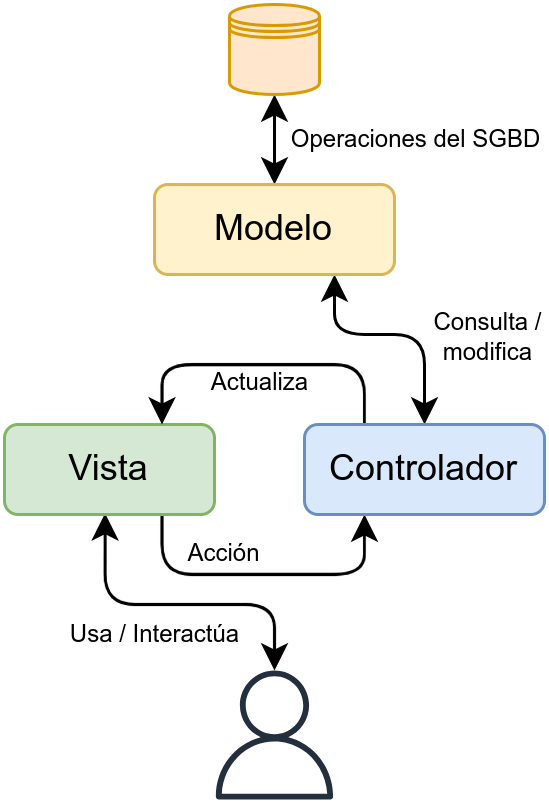
\includegraphics[width=\linewidth]{mvc.png}
\end{minipage}
}

\vspace{10pt}
Tal como se ha dicho, pueden existir distintas implementaciones, pero de manera generalizada y simplificada este sería el esquema básico de interacción.


\chapter{ORM}
Los sistemas ORM (del inglés \textit{Object-Relational mapping}, o “mapeo objeto-relacional”) es una técnica de programación para convertir los datos de una base de datos relacional en objetos cuando son utilizados en un lenguaje de programación orientado a objetos.

Este sistema “simula” una base de datos orientada a objetos (que no están muy extendidas) haciendo uso de las bases de datos relacionales que son ampliamente utilizadas y son más conocidas. De esta manera, también es un sistema menos a mantener.

Estos sistemas ORM suelen ocultar cómo se generan las peticiones a la base de datos, ya que para el programador lo único que hace es interactuar con objetos. El motor que usa Laravel se llama \href{https://laravel.com/docs/10.x/eloquent#retrieving-models}{Eloquent}.

Muchos \textit{framewors} de programación hacen uso de sistemas ORM, por lo que dependerá de cuál usemos podremos hacer uso de uno o podremos elegir entre varios. La wikipedia tiene una página donde se \href{https://en.wikipedia.org/wiki/List_of_object%E2%80%93relational_mapping_software}{listan distintos ORMs} separados por lenguajes de programación.

    \part{Crear entorno Laravel}
    \chapter{Crear primer proyecto en Laravel}

A la hora de crear un proyecto en Laravel lo primero que deberíamos hacer es visitar la \href{https://laravel.com/docs/10.x/installation}{documentación}, ya que nos dará distintas opciones dependiendo del sistema operativo en el que nos encontremos. Aparte, podremos ver si ha habido cambios desde la última vez que hayamos creado un proyecto.

\section{Servicios a utilizar}

Antes de crear el proyecto, debemos tomar una serie de decisiones para nuestro \textit{stack} de aplicación. Laravel cuenta con distintos servicios, algunos de ellos necesarios y otros optativos, por lo que deberemos tenerlos en cuenta.

Los servicios entre los que deberemos decidir son:

\begin{itemize}
    \item \textbf{Sistema Gestor de Base de Datos a utilizar}: Laravel permite el uso de distintos sistemas de bases de datos relacionales como son \href{https://dev.mysql.com/downloads/mysql/}{MySQL}, \href{https://www.postgresql.org/}{PostgreSQL} y \href{https://mariadb.org/}{MariaDB}. Por defecto hace uso de \textbf{MySQL}.
    \item \textbf{Sistema de caché}: Podemos hacer uso de distintos sistemas para cachear desde la sesión a información obtenida de la base de datos y también HTML. Por defecto, \textbf{Laravel cachea la sesión en el sistema de ficheros}, pero eso puede ser lento, por lo que se permite hacer uso de sistemas \textbf{clave-valor} para el almacenamiento de información para acelerar el rendimiento de la aplicación web. Se puede elegir \href{https://www.memcached.org/}{Memcached} o \href{https://redis.io/}{Redis} entre otros.
\end{itemize}

Otros servicios que podemos instalar y que nos darán ciertas funcionalidades son:

\begin{itemize}
    \item \textbf{\href{https://github.com/axllent/mailpit}{Mailpit}}: Es un sistema para controlar los emails que envía nuestra aplicación durante el desarrollo. En lugar de enviarlos a las cuentas finales, se quedan almacenados y se pueden visualizar a través de una web que a modo de buzón de correo. También ofrece una API.

    \item Uso de  \href{https://min.io/}{MinIO} para simular el \textbf{almacenamiento en la nube S3}. De esta manera no tendremos que crear un Bucket de pruebas.

    \item Sistema de \textbf{búsqueda \textit{full-text}} en la base de datos gracias a \href{https://laravel.com/docs/10.x/scout#introduction}{Scout} y haciendo uso del backend \href{https://www.meilisearch.com/}{MeiliSearch}.

    \item Creación y automatización de \textbf{tests} utilizando \href{https://www.selenium.dev/}{Selenium}.
\end{itemize}

Estas son algunas de los servicios que podríamos configurar antes de comenzar a crear nuestra aplicación. Para comenzar de manera sencilla nos centraremos únicamente en la elección de la base de datos, dejando el resto de servicios para más adelante.


\section{Instalación mediante Sail y Docker}

En la \href{https://laravel.com/docs/10.x/installation}{documentación} de Laravel nos explica cómo realizar la instalación de distintos modos teniendo en cuenta el sistema operativo, los servicios iniciales que nos interesan y el sistema de instalación que mejor se adapte a nuestro entorno.

%En este apartado se van a explicar dos modos:
%\begin{itemize}
%    \item Haciendo uso del método oficial y \textbf{Laravel Sail}, que nos permitirá elegir los servicios que necesitamos y que creará el proyecto haciendo uso de contenedores Docker.
%
%    \item Instalando Laravel utilizando \href{https://getcomposer.org/}{Composer}, que también es un método oficial, pero en este caso vamos a crear nosotros el contenedor Docker del servicio web y de base de datos. En caso de tener un entorno de PHP con Composer local, quizá no interesa realizar la creación del contenedor Docker.
%\end{itemize}
%
%Ambos métodos son igual de válidos y al final obtendremos un sistema similar.

%\subsection{}

El sistema es similar utilizando GNU/Linux, Windows y MacOS, con la salvedad de que en Windows deberíamos instalar Docker Desktop y \textit{Windows Subsystem for Linux} (WSL).

Para realizar la instalación sólo vamos a elegir tener el servicio de MySQL, para simplificarlo, tal como se ha comentado previamente. Para ello, deberemos ejecutar lo siguiente en el directorio donde nos interese crear el directorio del proyecto.

\begin{mycode}{Titulo}{console}{{\small }}
ruben@vega:~$ curl -s "https://laravel.build/example-app?with=mysql" | bash
\end{mycode}

Este comando lo que va a hacer es descargarse un script que va a ejecutar lo siguiente:
\begin{enumerate}
    \item Se va a asegurar que Docker está corriendo
    \item Va a levantar un contenedor con la imagen “laravelsail/php82-composer” que nos va a crear un directorio llamado \configdir{example-app} con un proyecto limpio de Laravel usando MySQL como SGBD.
    \item Si no tenemos la imagen de MySQL la descarga.
\end{enumerate}





\section{Configuración inicial}



%    \part{Laravel y Visual Studio Code como IDE}
    \chapter{Usar Visual Studio Code con Laravel}

\href{https://code.visualstudio.com/}{Visual Studio Code} es un entorno de desarrollo integrado (IDE) desarrollado por Microsoft y con licencia MIT, lo que lo hace Software Libre y que cualquiera pueda ver el código fuente, así como realizar modificaciones.

El problema es que Microsoft no ha liberado todo el código fuente, y los binarios que ofrece para descargar hacen uso de ese software, así como la inclusión de sistemas de telemetría. Es por eso que existe un proyecto llamado \href{https://vscodium.com/}{VSCodium} que ofrece los binarios libres de ese código.

Entre las ventajas que ofrece este IDE podemos destacar:

\begin{itemize}
    \item Se puede programar para muchos lenguajes de programación, no está especializado en uno sólo.

    \item Es extensible mediante \textit{plugins}. Hoy en día existen infinidad de extensiones para todo tipo de desarrollos.

    \item Es multiplataforma.

    \item Altamente configurable.

    \item Configurando la cuenta de GitHub, se puede sincronizar las configuraciones entre distintos dispositivos.

    \item Existe una versión \href{https://vscode.dev/}{online}.
\end{itemize}

\section{Extensiones recomendadas}

Para desarrollar con Laravel, aunque se puede extender a cualquier proyecto que haga uso de un entorno Docker, es recomendable utilizar una serie de extensiones para facilitar el desarrollo con ellos. De todas maneras, Visual Studio Code nos va a recomendar extensiones a medida que lo usemos, ya que observará el tipo de desarrollo que estamos realizando.

Entre las extensiones que se recomiendan están:
\begin{itemize}
    \item \href{https://marketplace.visualstudio.com/items?itemName=ms-vscode-remote.remote-containers}{Dev Containers}: Nos permite abrir un directorio o un repositorio que está dentro de un contenedor como si fuera local de nuestro equipo.

    \item \href{https://marketplace.visualstudio.com/items?itemName=onecentlin.laravel-extension-pack}{Laravel Extension Pack}: Es una “meta-extensión”, ya que incluye a otras extensiones creadas especialmente para ayudar durante el desarrollo de Laravel.
\end{itemize}

    \part{Añadir funcionalidad básica}
    \chapter{Introducción}

Ahora que ya tenemos el entorno creado, es momento de empezar a añadir funcionalidad básica a nuestra aplicación y comenzar a crear nuestra aplicación. Para estos ejemplos se ha decidido crear una pequeña aplicación a modo de blog, con posts y comentarios.

\chapter{Artisan}
\href{https://laravel.com/docs/10.x/artisan}{Artisan} es la interfaz de línea de comandos que vamos a utilizar para realizar todo tipo de interacción entre el proyecto y el propio \textit{framework} Laravel. Esta interfaz nos va a permitir, entre otras cosas:

\begin{itemize}
    \item Crear modelos y controladores.
    \item Crear una sesión a la base de datos.
    \item Controlar el estado de los “migrations”.
    \item Hacer uso de los “seeds” en la base de datos.
    \item Limpiar la caché de objetos.
\end{itemize}

Cada comando contará con su ayuda, por lo que es recomendable ir mirando la ayuda y así conocer las distintas opciones para cada uno de ellos.


\chapter{Crear modelo}
Un blog tiene una serie de “Posts”, que son las entradas que los usuarios introducen en el blog. De momento vamos a ignorar el apartado de usuarios, para simplificarlo. Una entrada del blog contará con los siguientes atributos:

\begin{itemize}
    \item Título
    \item Texto
    \item Si está publicada o no
\end{itemize}

Para crear el modelo, ejecutaremos el siguiente comando. Este comando lo debemos ejecutar dentro del contenedor Docker y dentro de la ruta donde se encuentra el proyecto Laravel, que es \configdir{/var/www/html}:

\begin{mycode}{Crear Modelo}{console}{}
root@1b29e46c10ae:/var/www/html# php artisan make:model Post -crms
\end{mycode}

Este comando nos va a crear el modelo Post junto con:
\begin{itemize}
    \item \textbf{Controlador} de tipo “resource”, lo que va a permitir realizar acciones “\textbf{CRUD}” (\textit{create}, \textit{read}, \textit{update} y \textit{delete}), necesarias en cualquier aplicación web.
    \item \textbf{\textit{Migration}}: Un fichero para realizar la migración del modelo en la base de datos.
    \item \textbf{\textit{Seed}}: Un fichero de tipo “semilla” para introducir datos en la base de datos.
\end{itemize}

\chapter{Entendiendo las “\textit{migrations}” de base datos}

Hoy en día son muchos los \textit{frameworks} que hacen uso de sistemas de tipo \textbf{\textit{migration}} a la hora de interactuar en el tiempo con la base de datos. Podríamos definirlo como un \textbf{sistema de control de versiones para el esquema de base de datos}.

Este sistema permite ir evolucionando el esquema de base de datos (tablas, columnas de las tablas, funciones...) a medida que el propio código fuente de la aplicación va evolucionando. De esta manera, si tenemos el código en un punto concreto, con el sistema \textbf{migrations} nos va a crear la base de datos tal como se necesita en ese punto.

Al crear nuestro proyecto Laravel, ya contamos con una serie de ficheros de migraciones para la base de datos. Estos ficheros se encuentran en \configdir{app/database/migrations/}, teniendo cada fichero un formato similar a \configfile{YYYY_mm_dd_HHMMSS_comentario.php} siendo:

\begin{itemize}
    \item \textbf{YYYY}: el año que se ha creado el fichero.
    \item \textbf{mm}: el mes que se ha creado el fichero.
    \item \textbf{dd}: el día que se ha creado el fichero.
    \item \textbf{HHMMSS}: la hora, minuto y segundo.
    \item \textbf{comentario}: un pequeño comentario sobre el contenido del fichero.
\end{itemize}

De esta manera, los migrations se van a poder ejecutar en orden de fecha de creación, donde normalmente suele ser:
\begin{itemize}
    \item \textbf{De más antiguo a más nuevo}: Se van creando las tablas, y se van añadiendo modificaciones. Es el ciclo normal de de desarrollo, y este es el sistema de uso habitual.
    \item \textbf{De más nuevo a más antiguo}: Se vuelve atrás en el proyecto, eliminando modificaciones. Utilizado para ir a una versión antigua del proyecto.
\end{itemize}

Vamos a utilizar como ejemplo el primer fichero que existe en el directorio, que es para hacer uso de la tabla de usuarios del sistema de autenticación de Laravel. El fichero tiene una clase que extiende de la clase \textbf{Migration} con dos funciones:

\begin{mycode}{Fichero Migration}{PHP}{}
<?php
use Illuminate\Database\Migrations\Migration;
use Illuminate\Database\Schema\Blueprint;
use Illuminate\Support\Facades\Schema;

return new class extends Migration {
    public function up(): void {
        Schema::create('users', function (Blueprint $table) {
            $table->id();
            $table->string('name');
            $table->string('email')->unique();
            $table->timestamp('email_verified_at')->nullable();
            $table->string('password');
            $table->rememberToken();
            $table->timestamps();
        });
    }

    public function down(): void {
        Schema::dropIfExists('users');
    }
};
\end{mycode}

La función \inlineconsole{up()} se ejecutará cuando realizamos la migración, mientra que la función \inlineconsole{down()} se usará cuando realicemos un “\textbf{\textit{rollback}}” (echar para atrás una migración).


\warnbox{\textbf{Por convenio, el nombre de los modelos suelen ser en singular, mientras que las tablas se deben crear en plural. \href{https://laravel.com/docs/10.x/eloquent\#table-names}{Pero se puede cambiar el nombre de la tabla}.}}

\section{Opciones de las migraciones}

En la \href{https://laravel.com/docs/10.x/migrations#tables}{documentación oficial} se explican cómo funcionan los \textit{migrations} y las funcionalidades básicas y avanzadas que tienen.

Teniendo en cuenta lo visto en el punto anterior, podemos visualizar que las acciones del \textit{migration} contiene varias líneas, y vamos a destacar lo siguiente para el fichero \configfile{2014_10_12_000000_create_users_table.php}:

\begin{itemize}
    \item Crea una tabla llamada “\textbf{users}”, que contiene varias columnas
    \item \textbf{id}: es un alias al método \textbf{bigIncrements}. Va a generar una columna de tipo “\textit{big integer}” sin signo, que se va a ir incrementando y que va a ser \textbf{clave primaria}.

    \item \textbf{string}: existen varias columnas de tipo “string”, que son “name”, “email” y “password”. Es lo equivalente a “varchar”, sin indicar en este caso el número de longitud. Se le puede indicar como segundo parámetro.
    \item \textbf{unique()}: el contenido de este campo (en el ejemplo el \textbf{email}) debe ser único en la tabla.
    \item \textbf{timestamp}: crea un campo de tipo TIMESTAMP.
    \item \textbf{nullable}: permite que este campo sea \textbf{null}.

    \item \textbf{timestamps()}: Este es un método especial que crea dos campos en la base de datos: “\textbf{created\_at”} y “\textbf{updated\_at}”. De esta manera sabemos cuándo se ha creado y modificado el registro en la base de datos.
\end{itemize}

\exercisebox{Añade a la migración del modelo Post, la generación de los campos: “título”, “texto” y “publicado”. Recuerda mirar la documentación oficial.}

\section{Uso de las migraciones}

Una vez tenemos distintos ficheros de migraciones, hay que saber cómo aplicarlos y qué sucede con ellos. De nuevo, en la \href{https://laravel.com/docs/10.x/migrations#running-migrations}{documentación} aparecen distintos ejemplos, de los cuales se van a destacar sólo unos a continuación:

\subsection{Desplegar migraciones}
Para realizar el despliegue de todas las migraciones debemos ejecutar el siguiente comando:

\begin{mycode}{Ejecutar migraciones}{console}{}
root@1b29e46c10ae:/var/www/html# php artisan migrate
   INFO  Preparing database.
Creating migration table ............................. 52ms DONE

   INFO  Running migrations.
2014_10_12_000000_create_users_table ..............   108ms DONE
2014_10_12_100000_create_password_reset_tokens_table  127ms DONE
2019_08_19_000000_create_failed_jobs_table .........   88ms DONE
2019_12_14_000001_create_personal_access_tokens_table 140ms DONE
2023_09_26_094514_create_posts_table ...............   74ms DONE
\end{mycode}

\subsection{Comprobar estado de las migraciones}

Para comprobar el estado de las migraciones podemos realizarlo de la siguiente manera:
\begin{mycode}{Estado de las migraciones}{console}{}
root@1b29e46c10ae:/var/www/html# php artisan migrate:status

Migration name ................................ Batch / Status
2014_10_12_000000_create_users_table ................. [1] Ran
2014_10_12_100000_create_password_reset_tokens_table . [1] Ran
2019_08_19_000000_create_failed_jobs_table ........... [1] Ran
2019_12_14_000001_create_personal_access_tokens_table  [1] Ran
2023_09_26_094514_create_posts_table ................. [1] Ran
\end{mycode}


Si queremos ver a nivel de base de datos qué ha pasado, podemos ejecutar una sesión y visualizar la propia base de datos. Veremos cómo se ha creado la base de datos, las tablas, y una tabla especial llamada \textbf{migrations}, que contiene qué ficheros se han desplegado.

\begin{mycode}{Ejecutar migraciones}{mysql}{}
root@1b29e46c10ae:/var/www/html# php artisan db

mysql> use example_app;
Database changed

mysql> show tables;
+------------------------+
| Tables_in_example_app  |
+------------------------+
| failed_jobs            |
| migrations             |
| password_reset_tokens  |
| personal_access_tokens |
| posts                  |
| users                  |
+------------------------+
6 rows in set (0.00 sec)

mysql> select * from migrations;
+----+-------------------------------------------------------+-------+
| id | migration                                             | batch |
+----+-------------------------------------------------------+-------+
|  1 | 2014_10_12_000000_create_users_table                  |     1 |
|  2 | 2014_10_12_100000_create_password_reset_tokens_table  |     1 |
|  3 | 2019_08_19_000000_create_failed_jobs_table            |     1 |
|  4 | 2019_12_14_000001_create_personal_access_tokens_table |     1 |
|  5 | 2023_09_26_094514_create_posts_table                  |     1 |
+----+-------------------------------------------------------+-------+
5 rows in set (0.00 sec)
\end{mycode}


\subsection{\textit{Rollback} la última migración}

En un momento dado nos puede interesar echar atrás la última migración, y para ello contamos con la opción \textbf{\textit{rollback}}. Este sistema puede que deshaga las migraciones de varios ficheros.

\begin{mycode}{Ejecutar migraciones}{mysql}{}
root@1b29e46c10ae:/var/www/html# php artisan migrate:rollback

INFO  Rolling back migrations.
2023_09_26_094514_create_posts_table ................  27ms DONE
2019_12_14_000001_create_personal_access_tokens_table  26ms DONE
2019_08_19_000000_create_failed_jobs_table ..........  25ms DONE
2014_10_12_100000_create_password_reset_tokens_table   24ms DONE
2014_10_12_000000_create_users_table ................  27ms DONE
\end{mycode}

En este caso, como el migrate hizo todos los ficheros, el \textit{rollback} se ha ejecutado de todos los ficheros pero \textbf{en orden inverso al de creación}.


\subsection{Limpiar, \textit{reset} y recarga de migraciones}

Para asegurar que el sistema de migraciones está funcionando bien, para hacer pruebas, o para realizar despliegues limpios quizá nos interese borrar todas las migraciones de la aplicación o realizar una recarga de las mismas.

\begin{itemize}
    \item \textbf{db:wipe}: borra todas las tablas, vistas y tipos.
    \item \textbf{migrate:fresh}: borra todas las tablas de la base de datos y aplica de nuevo todas migraciones.
    \item \textbf{migrate:reset}: deshace todas las migraciones de la aplicación. Básicamente es dejar la base de datos limpia. \textbf{En este caso no se borra la tabla “\textit{migration}”}.
    \item \textbf{migrate:refresh}: deshace todas las migraciones de la aplicación y las vuelve a aplicar en orden.
\end{itemize}


\section{Uso de las semillas}

A la hora de crear una aplicación es posible que nos interese que tras realizar un primer despliegue existan datos en la base de datos. Ya sea porque estos datos son necesarios para el correcto funcionamiento de la aplicación o para darle una funcionalidad básica.

Para poblar de datos la base de datos existe el sistema de semillas, o \textbf{\textit{seeds}}. Este sistema funciona a través de sus propios ficheros, que se pueden crear por modelo (tal como hemos hecho en este capítulo), o de manera general en una semilla propia.

Con la generación del modelo se ha creado también el fichero  al que vamos a añadirle el código necesario para que cree un primer post de pruebas: \configfile{app/database/seeders/PostSeeder.php}.

\begin{mycode}{\textit{Seed} del PostSeeder.php}{php}{}
<?php
use Illuminate\Database\Console\Seeds\WithoutModelEvents;
use Illuminate\Database\Seeder;
use Illuminate\Support\Facades\DB;

class PostSeeder extends Seeder {
    public function run(): void {
        DB::table('posts')->insert([
            "titulo"=>"Primer post",
            "texto"=>"Este es el texto del primer post",
            "publicado"=>true,
            "created_at"=>now(),
        ]);
    }
}
\end{mycode}

Para poder hacer uso del modelo “\textbf{DB}” es necesario hacer uso de la librería \configfile{Illuminate\Support\Facades\DB}. Ahora sólo queda ejecutar el \textit{seed} tal como se explica en la \href{https://laravel.com/docs/10.x/seeding}{documentación}:

\begin{mycode}{Ejecutar el seed}{console}{}
root@1b29e46c10ae:/var/www/html# php artisan db:seed PostSeeder
INFO  Seeding database.
\end{mycode}

Si se comprueba la base de datos, se verá cómo en la tabla aparecen los datos del \textit{seed}.


\chapter{Rutas de la aplicación}

Aunque ya tenemos un controlador y datos en la aplicación, hasta ahora son inaccesibles. Lo único que vemos en la aplicación es la página de bienvenida al proyecto y si ponemos cualquier ruta en la URL nos aparece un error “404 Not Found”.

Esto es debido al sistema de enrutado de la aplicación, que sólo permite acceder al \textit{path} “/” que nos muestra la plantilla de bienvenida. Esta configuración se puede ver en el fichero \configfile{routes/web.php}.

\begin{mycode}{Rutas de la aplicación web de Laravel}{php}{}
<?php
use Illuminate\Support\Facades\Route;

Route::get('/', function () {
    return view('welcome');
});
\end{mycode}

Cualquier intento de acceso a algo que no sea esa ruta dará un error 404. Este es un sistema de seguridad para controlar a qué se tiene acceso en la aplicación, y por eso que debemos modificar este fichero para poder acceder a nuestro nuevo controlador.

\begin{mycode}{Añadiendo rutas para el nuevo controlador}{php}{}
<?php
// ...
use App\Http\Controllers\PostController;
Route::controller(PostController::class)->group(function () {
    Route::get('/posts', 'index')->name('posts.index');
    Route::get('/posts/{post}', 'show')->name('posts.show');
});
\end{mycode}

Este código indica que se va a utilizar la clase “PostController” para el grupo de las rutas que aparecen en ese trozo de código. Si vamos al fichero \configfile{App\Http\Controllers\PostController.php} veremos que por defecto todas las funciones están vacías, y es por eso que no nos devuelve ningún dato.

Por lo tanto, la idea es:

\begin{itemize}
    \item \textbf{/posts}: irá a la función “index” del controlador. Esta función normalmente lista el contenido de la tabla de base de datos que hace referencia al modelo. En nuestro caso, mostrará todos los posts del blog (normalmente en formato paginado).
    \item \textbf{/posts/\{post\}}: esta ruta será la utilizada cuando queramos ir a ver un registro del modelo concreto. En este caso “\{post\}” indicará el “id” dentro de la base de datos que se le pasará a la función “show”.
\end{itemize}

En el siguiente apartado, cuando modifiquemos el controlador quedará más claro.

\section{Tipos de rutas}

Hay que entender que las rutas funcionan en base al protocolo HTTP. Esto quiere decir que existen distintas maneras de acceder a la misma URL dependiendo del tipo de petición que se realice en base a lo que realicemos con el navegador.

Normalmente, cuando navegamos por internet, las peticiones que se realizan son de tipo \textbf{GET}, ya que estamos pidiendo información al servidor web. En cambio, cuando rellenamos un formulario y le damos a enviar, se hace uso del “verbo” \textbf{POST}, ya que se envían datos al servidor.

Las peticiones HTTP que se pueden utilizar son:

\begin{itemize}
    \item \textbf{GET}: Se realiza una petición a la ruta especificada. Estas peticiones sólo obtienen información.
    \item \textbf{POST}: Se envían datos al servidor, que van incluidos dentro del cuerpo de la petición. Lo habitual cuando utilizamos formularios. Se utiliza para crear nuevos recursos.
    \item \textbf{PUT}: Similar a POST, pero en este caso suele estar orientado a modificar datos previamente creados.
    \item \textbf{PATCH}: Como PUT, sobreescribe completamente un recurso existente.
    \item \textbf{DELETE}: Borra el recurso especificado.
\end{itemize}

Es conveniente mirar la \href{https://laravel.com/docs/10.x/routing}{documentación} cuando queramos realizar algún tipo de petición distinto de GET, ya que nos ayudará a comprender mejor qué es lo que está sucediendo.

\chapter{Controladores y Vistas}
Ahora que ya tenemos las rutas creadas, es momento de que los datos se visualicen en la aplicación. Para ello es necesario entender cómo funciona el sistema de plantillas utilizado por Laravel, llamado \textbf{\href{https://laravel.com/docs/10.x/blade}{Blade}}, que junto con el sistema de \textbf{enrutado} visto previamente, relaciona la URL a la que se llama con el controlador y la vista correspondientes.

\section{Obtener datos en el controlador}

El ejemplo va a consistir en obtener todos los posts de la base de datos y hacer un listado con ellos. Por otro lado, al seleccionar un post concreto, se mostrará dicho post. Para ello vamos a modificar el controlador para modificar las dos funciones que se utilizan en las rutas:

\begin{mycode}{Funciones modificadas en el controlador Post}{php}{}
<?php
// ...
use App\Models\Post;
// ...
class PostController extends Controller{
    public function index(){
        $posts = Post::orderBy('created_at')->get();
        return view('posts.index',['posts' => $posts]);
    }
    //...
    public function show(Post $post){
        return view('posts.show',['post'=>$post]);
    }
\end{mycode}

El problema de este código es que estamos llamando a unas vistas que todavía no hemos creado, y les estamos pasando como variables a la vista los datos obtenidos dentro de un array. Podremos pasar tantas variables como queramos.


\section{Generar vista}

El sistema de plantillas y vistas Blade se guardan en la ruta \configdir{resources/views}, y en el primer caso lo que estamos diciendo es que haga uso de “posts.index”, que quiere decir el fichero “index.blade.php” del directorio “posts”. Por lo tanto, deberemos crear un fichero en la ruta \configfile{resources/views/posts/index.blade.php}, que corresponde a la vista que estamos llamando.

\infobox{\textbf{Es recomendable para cada Modelo/Controlador crear un directorio de vistas}}

Ahora es momento de visualizar los datos en la vista. Para ello, recorreremos el listado obtenido y lo visualizaremos, todo ello en la vista. El sistema de plantillas \href{https://laravel.com/docs/10.x/blade}{Blade} permite introducir funcionalidad similar a PHP en la vista mezclado con HTML. También permite incrustar código PHP directamente, pero intentaremos evitarlo.

El sistema de plantillas tiene una serie de palabras reservadas similar a la de los lenguajes de programación más habituales. En este ejemplo se va a recorrer con un bucle for la lista, se crea una variable de indexación, y así poder visualizar los atributos:

\begin{mycode}{Vista “index.blade.php”}{html+smarty}{}
<ul>
  {{--esto es un comentario: recorremos el listado de posts--}}
  @foreach ($posts as $post)
    {{-- visualizamos los atributos del objeto --}}
    <li>
      <a href="{{route('posts.show',$post)}}"> {{$post->titulo}}</a>.
      Escrito el {{$post->created_at}}
    </li>
  @endforeach
</ul>
\end{mycode}

Si ahora visualizamos la ruta “/posts” obtendremos el listado. Es importante destacar que para el enlace que nos lleva a visualizar un post concreto \textbf{se ha hecho uso del sistema ed rutas} al que se le pasa como parámetro el post.

\exercisebox{Crea la vista para visualizar toda la información del post en “show.blade.php”.}


\chapter{\textit{Soft Deleting}}

Laravel, a través de su ORM Eloquent, nos permite hacer uso del sistema “\textit{\href{https://laravel.com/docs/10.x/eloquent\#soft-deleting}{soft deleting}}”, que en lugar de borrar los registros de la base de datos, lo que hace es marcarlo como borrado. Esto lo hace a través de una columna en la base de datos, indicando con una fecha cuándo se ha borrado.

Es habitual hacer uso de estos sistemas, por si el borrado ha sido erróneo, y de esta manera poder recuperar registros (ya que realmente no se han borrado).

Para hacer uso de este sistema debemos indicarlo en el modelo, para ello le indicaremos que se va a usar “\textbf{SoftDeletes}”:

\begin{mycode}{Indicar en el modelo el uso de Softdeletes}{php}{}
<?php
//...
use Illuminate\Database\Eloquent\SoftDeletes;
class Post extends Model{
    use SoftDeletes;
    //...
}
\end{mycode}

Y también debemos indicarlo en la generación de la base de datos (o en un nuevo \textit{migration}). De esta manera, se creará la columna correspondiente que es necesaria.

\begin{mycode}{Indicar en el “migration” el uso de Softdeletes}{php}{}
<?php
//...
public function up(): void {
    Schema::create('posts', function (Blueprint $table) {
        $table->id();
        $table->string("titulo",128);
        $table->string("texto",5000);
        $table->boolean("publicado");
        $table->softDeletes();
        $table->timestamps();
    });
}
\end{mycode}

Si ejecutamos los \textit{migrations}, veremos que la tabla tiene un campo “\textbf{deleted\_at}”, que por defecto estará a NULL. Si ahora borramos un registro, se actualizará esa columna con la fecha del momento en el que se ha realizado la acción de borrado. \textbf{Estos registros pueden ser recuperados}.



\chapter{Debug}
Durante el desarrollo es habitual hacer uso de sistemas de \textit{debug}, por ejemplo para poder ver el contenido de variables y parar la ejecución del algoritmo que estamos programando.

Laravel cuenta con una función llamada \inlineconsole{dd()} que podemos utilizar en cualquier momento. Por ejemplo, si lo usamos en el controlador creado previamente:

\begin{mycode}{Llamar a Tinker con Artisan}{php}{}
<?php
 public function index(){
    $posts = Post::all();
    dd($posts);
    return view('posts.index',['posts' => $posts]);
}
\end{mycode}

En este caso, se ejecutará la petición de obtener todos los \textit{posts}, y acto seguido la función \inlineconsole{dd($posts)} lo que hará será mostrar por pantalla el contenido de la variable y terminará la ejecución del código.


\chapter{Consola Tinker}

Hoy en día muchos \textit{frameworks} tienen algún sistema de consola interactiva con la que poder utilizar las funcionalidades del mismo. De esta manera, podemos realizar comprobaciones, interactuar con los modelos, objetos... pero sin tener que hacerlo desde el código de la web.

En el caso de Laravel la consola se llama \href{https://laravel.com/docs/10.x/artisan#tinker}{Tinker}, y se puede llamar de dos maneras, dependiendo desde dónde lo hagamos:
\begin{itemize}
    \item Si lo realizamos desde dentro del contenedor, usaremos Artisan de la siguiente manera:
\begin{mycode}{Llamar a Tinker con Artisan}{console}{}
root@1b29e46c10ae:/var/www/html# php artisan tinker
Psy Shell v0.11.21 (PHP 8.2.10 — cli) by Justin Hileman
\end{mycode}

    \item Si lo hacemos desde nuestro servidor anfitrión, usaremos Sail:
\begin{mycode}{Arrancamos los servicios}{console}{}
ruben@vega:~$ cd example-app && ./vendor/bin/sail tinker
Psy Shell v0.11.21 (PHP 8.2.10 — cli) by Justin Hileman
\end{mycode}
\end{itemize}

Una vez dentro, podremos hacer uso de los modelos, por ejemplo, para ver los datos que tenemos en la base de datos.

\begin{mycode}{Arrancamos los servicios}{psysh}{}
> Post::all();
[!] Aliasing 'Post' to 'App\Models\Post' for this Tinker session.
= Illuminate\Database\Eloquent\Collection {#7247
    all: [
    App\Models\Post {#7249
        id: 1,
        titulo: "Primer post",
        texto: "Este es el texto del primer post",
        publicado: 1,
        created_at: "2023-10-01 16:57:30",
        updated_at: null,
    },
    ],
}
\end{mycode}


        %Cómo crear una API con Laravel
    %     - crear proyecto
    %    - crear esquema E/R
    %    - crear controlador
    %    - crear funciones

\end{document}